\input{../../input/main}

\begin{document}

\begin{center}
  \Large{\textbf{Городской центр физического образования, 10 класс.}\\
  \textit{Серия 8Ш, 17 ноября 2014.}}
\end{center}

\begin{center}
  \Large\textbf{ Районный тур уже близко: электричество. }
\end{center}

\large

\taskpic{ Для бытовых нужд была изготовлена модель часов с
  подсветкой. Центр циферблата подключен через источник питания к
  точке на его ободе, соответствующей времени 12–00. Обе стрелки часов
  проводят электрический ток и касаются своими концами обода
  циферблата, при этом сопротивление минутной стрелки в три раза
  больше, чем сопротивление часовой. Сам обод тоже состоит из
  проводящего материала, однородного по всей длине, который светится,
  когда по нему проходит сколь угодно малый электрический ток. На
  часах полночь. Укажите все моменты времени, в которые не весь обод
  циферблата будет светиться. }
{
  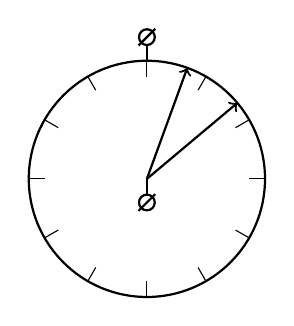
\begin{tikzpicture}
    \draw[thick] (0,0) circle (1.5cm);
    \foreach \i in {0,1,2,...,11}
    {
      \draw[rotate around={30*\i:(0,0)}] (1.3,0) -- (1.5,0); 
    }
    \draw[thick,->] (0,0) -- ++(40:1.5cm);
    \draw[thick,->] (0,0) -- ++(70:1.5cm);
    \draw[thick] (0,0) -- ++ (0,-0.2cm);
    \draw[thick] (0,-0.3) circle (0.1cm);
    \draw[thick] (0,-0.3) ++(45:0.15cm) -- ++(225:0.3cm);
    \draw[thick] (0,1.5cm) -- ++(0,0.2cm);
    \draw[thick] (0,1.8cm) circle (0.1cm);
    \draw[thick] (0,1.8cm) ++(45:0.15cm) --++(225:0.3cm);
  \end{tikzpicture}
}
% СПб, район-10, 2012

\taskpic[5cm]{ Схема, приведённая на рисунке, содержит два ключа и
  пять одинаковых лампочек. Схема подключена к источнику постоянного
  напряжения. Считая, что изначально все ключи замкнуты, расположите
  лампочки в порядке возрастания яркости. В каком положении должны
  находиться ключи $K_1$ и $K_2$, чтобы лампочка №4 горела с
  минимально возможной яркостью? Ответы обоснуйте. }
{
  \begin{tikzpicture}[circuit ee IEC,thick]
    \node[contact] (1) at (0,2.5) {};
    \node[contact] (2) at (0,0) {};
    \node[contact] (3) at (2.5,2.5) {};
    \node[contact] (4) at (2.5,0) {};
    \draw[thick] (2) to[bulb={near start}] (3);
    \draw[thick] (1) to[bulb={info={\small $\mbox{Л}_1$}}] (3)
    to[bulb={info'={\small $\mbox{Л}_2$}} ] (4)
    to[bulb={info={\small $\mbox{Л}_3$}}] (2) to[bulb={info={\small
        $\mbox{Л}_5$}}] (1); 
    \draw[draw=white,double=black,double distance=\pgflinewidth,ultra
    thick] (1) to[make contact={near end}] (4);
    \draw[thick] (3) -- ($(3)+(0.5,0)$) to[make
    contact={info={\small $K_1$}}] ($(4)+(0.5,0)$) -- (4);
    \node (L4) at (0.6,1.1) {\small $\mbox{Л}_4$};
    \node (K2) at (1.6,0.5) {\small $K_2$};
    \draw[o-] ($(1)+(-0.5,0)$) -- (1);
    \draw[o-] ($(2)+(-0.5,0)$) -- (2);
  \end{tikzpicture}
}
% СПб, район-10, 2009

\taskpic[5cm]{ Электрическая схема, представленная на рисунке, состоит из
  2014 секторов. Каждое ребро сектора представляет собой резистор
  сопротивлением 1 Ом. Определите сопротивление между точками
  \textbf{A} и \textbf{B} в схеме. }
{
  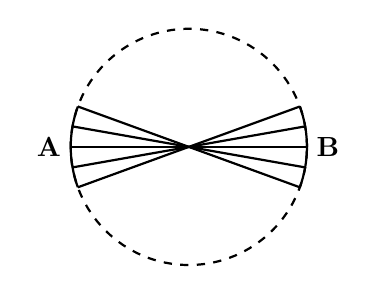
\begin{tikzpicture}
    \draw[dashed,thick] (0,0) circle (1.5cm);
    \foreach \i in {-2,-1,...,2}
    {
      \draw[thick] (0,0) ++(\i*10:1.5cm) -- (180+\i*10:1.5cm); 
    }
    \draw[thick] (0,0) ++(-20:1.5cm) arc (-20:20:1.5cm);
    \draw[thick] (0,0) ++(200:1.5cm) arc (200:160:1.5cm);
    \draw (-1.5,0) node[left] {\textbf{A}};
    \draw (1.5,0) node[right] {\textbf{B}}; 
  \end{tikzpicture}
}

\end{document}
% СПб, район-10, 2008

%%% Local Variables: 
%%% mode: latex
%%% TeX-engine:xetex
%%% TeX-PDF-mode: t
%%% End:
